\chapter{\label{chap:Phoneme-Split}Phoneme Split}

In this chapter we will develop a model of phoneme split, or genesis,
using the phenomenon of vowel nasalization as a case study. The model
will be based on the analyses of the preceding chapters: the metric
of success will be representational consistency and stability, with
the ability to achieve multiple stable states under different parameter
settings. The relevant parameters will also be required to serve as
testable hypotheses about possible actuation mechanisms. The first
of two model variants, the No-Phoneme Model will contain explicit
representations only at the word-level, and will be used primarily
to illustrate a particular implementation of the frequency effect.
The subsequent model, the Multiple-Parse Model will add a sub-lexical
level of analysis. The major innovation of this model will be an explicit,
non-one-to-one, perception-to-production mapping in which the likelihood
of a given analysis depends on the phonetic properties of the input.
Additionally, no analysis is taken to be more `correct' than any other,
just as the set of possible sub-lexical units is not taken to determined
ahead of time.

\section{Representations I}

It has been well-established in both perception and production that
a negative correlation between degree of vowel nasalization and strength
of nasal consonant exists (e.g., \citealt{kawasaki1978perceived,cohn1990phonetic}).
This is consistent with the hypothesis that the final nasal is more
likely to be lost, the more nasalized the preceding vowel becomes.
A possible explanation can be found in a listener-oriented theory
of change, where speakers strive to preserve acoustic cues for ease
of listener comprehension. Strong nasal cues on the vowel predict
the upcoming nasal, which means that speakers may expend less effort
to preserve the actual nasal, allowing it to erode. As with other
proposals, the question that still remains to be answered is how the
vowel came to have such strong nasal cues in the first place (presumably
stronger than the typical range of phonetic nasalization observed
cross-linguistically). 

A different perspective will be adopted here, building on the observation
of \citet{Beddor2009} that the negative correlation between vowel
nasality and consonant nasality follows directly from a single articulatory
parameter: the degree of overlap of the vowel and nasal gestures.
The more overlap, the greater the extent of nasalization on the vowel,
and the shorter the duration of the purely consonantal nasal, and
vice versa (see Fig. \ref{fig:Normal nasalization}). It will be assumed
that successful production requires stored articulatory targets, and
that these must be inferred from acoustic inputs. For simplicity,
only a single word type will be modeled, that consisting of a tongue
body gesture followed by a velum gesture (e.g., “am”). The production-perception
mapping will take place over three phonetic variables: duration of
tongue body gesture, duration of velum gesture, and duration of gestural
overlap $(x^{V},x^{N},x^{O})$. Categorization will occur at the level
of the word, and does not require decomposition into phonemes. Thus,
these models will not assume that there exists an allophonic process
of vowel nasalization. The initial distributions for all tokens will
be generated by independent sampling from three separate Normal distributions,
corresponding to $x^{V}$, $x^{N}$, and $x^{O}$, respectively. 

In Chapter \ref{sec:Models-of-Change} we saw that (soft) targets
were needed to constrain the basic exemplar model of change. What
this did was effectively force an independent production component
into a model which otherwise equated acoustic and articulatory representations.
In the current set of models this is not necessary, implementationally,
or conceptually, because each acoustic token has its own production
target. This is depicted schematically in Fig. \ref{fig:P-toP-mapping},
where stored articulatory parameters (represented by temporally overlapping
articulatory gestures) are realized as acoustic tokens during production
(dark patterned rectangles representing sound frequency information
over time), and acoustic tokens are, in their turn, transformed into
stored articulatory parameters during perception. At the word level,
this is a \noun{state} model; the articulatory variables are stored
without normalization. At the gestural level, however, there is the
possibility of an implicit \noun{process} model in the fact that the
overlap dimension represents the concatenation of two units, as well
as the source of nasalization. We will return to this point below.

\begin{figure}[H]

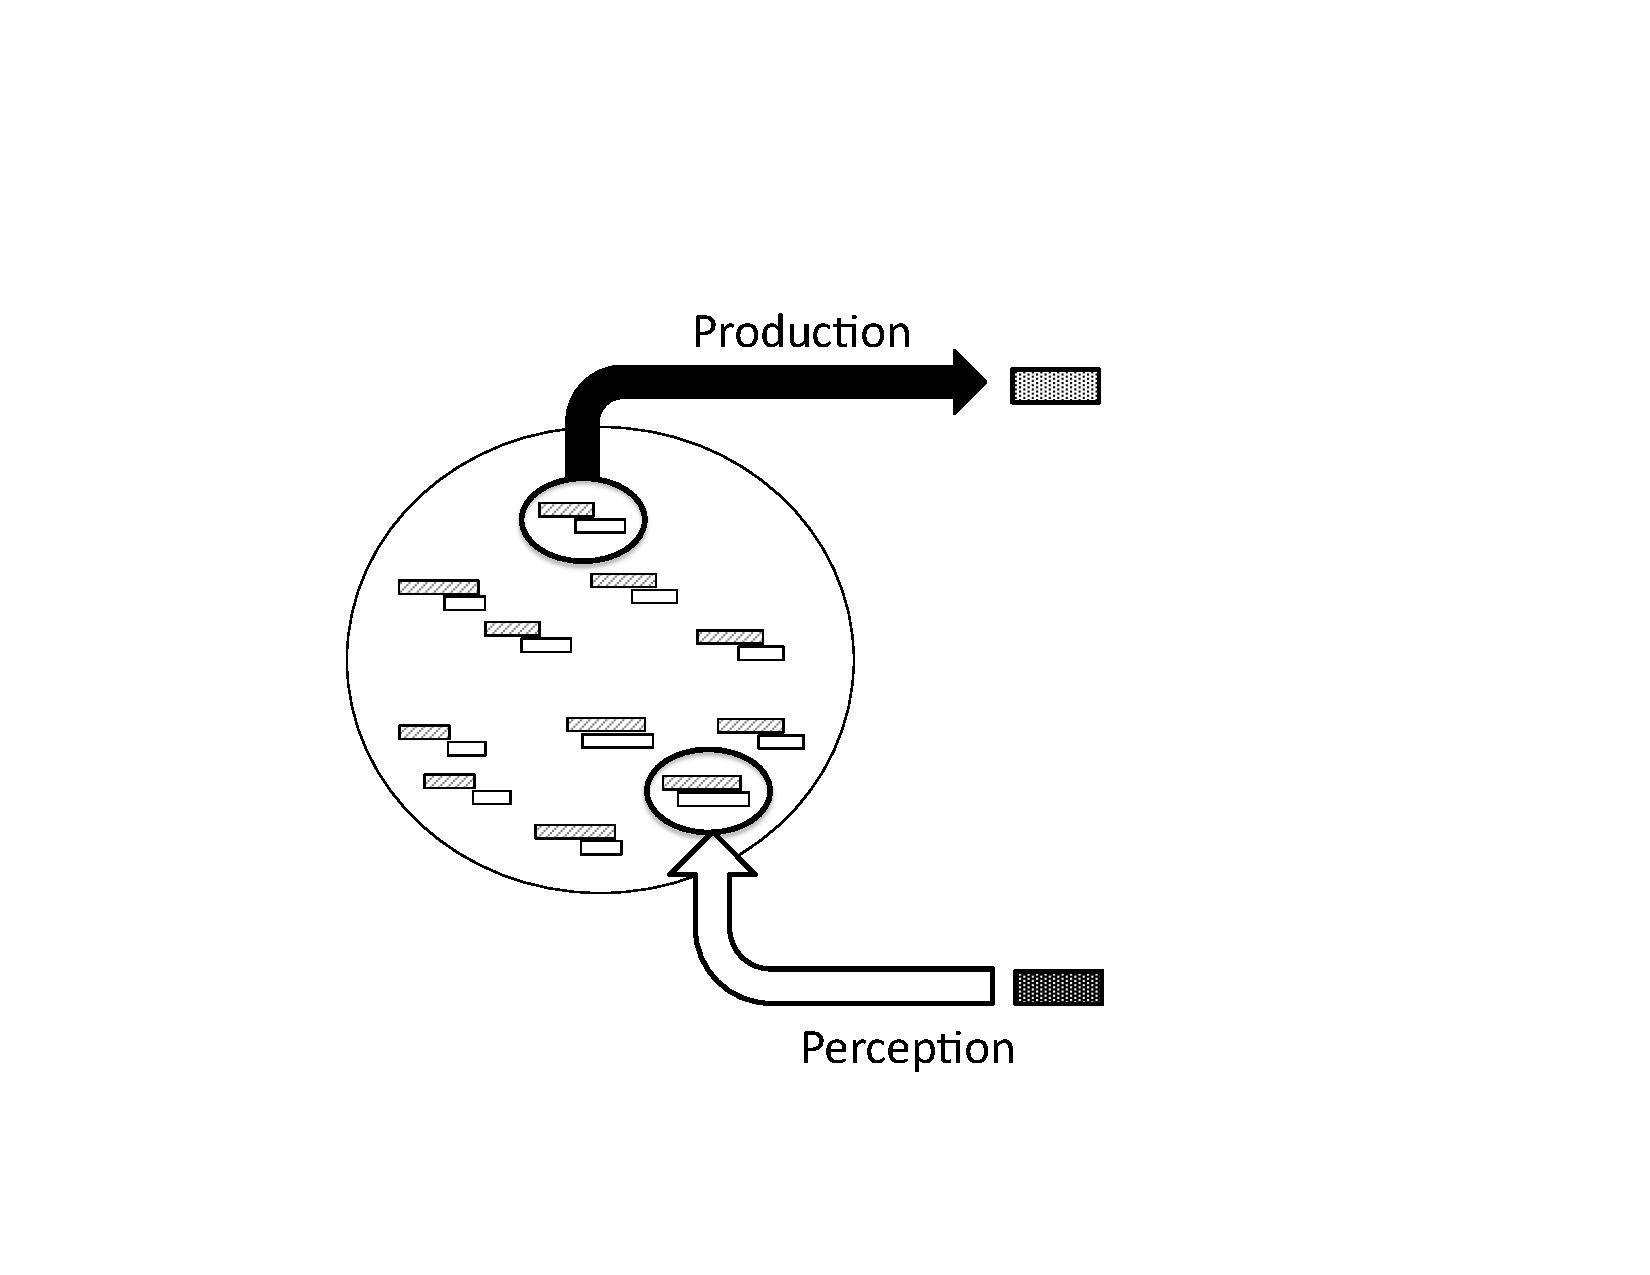
\includegraphics[width=0.75\textwidth,bb = 0 0 200 100, draft, type=eps]{SeparateReps.pdf}\caption{\label{fig:P-toP-mapping}Graphical depiction of an explicit mapping
between articulatory representations and acoustic representations. }

\end{figure}

As Chapter \ref{sec:Model-Behavior} showed, the two-attractor (\noun{state}
model) had a limited range of output states: the entire distribution
always stabilizes at some point intermediate between the two attractors.
Furthermore, that model contained no mechanism for changing the attractor
locations, or introducing new attractors. The current model effectively
explodes the number of attractors (or underlying representations)
to the number of tokens within a category. This allows for more complex
model dynamics. It also allows for changes to occur to the attractors
themselves, via independent forces that act, not at the level of the
word (or at the level of the phoneme), but at the level of the gestural
variables. Individual tokens of a given word category can thus be
altered, with the possibility, but not the guarantee, that such changes
can spread throughout the entire distribution of tokens.

\section{\label{sec:Frequency-I}Frequency I}

The first iteration of the phoneme-split model uses a frequency-based
attractor as the actuator of change. Based on the assumption that
frequency-based reduction is the result of increased fluency, and
that to be fluent is to produce some (nearly) ideal balance of efficiency
and intelligibility, an optimal degree of gestural overlap, \emph{T},
is defined. Relative word frequency is implemented as a parameter
($\beta$; $0<\beta<1$) that controls the degree to which each token
of the category is shifted towards the target, \emph{T}, during production.
Thus, for a stored production token consisting of the duration triple
$(x_{i}^{V},x_{i}^{N},x_{i}^{O})$, a fluency effect applies to the
ultimate realization of $x_{i}^{O}$, the gestural overlap value,
in the following way: 

\begin{equation}
Fluency:x_{i}^{O^{\prime}}=x_{i}^{O}+\beta(T-x_{i}^{O})\label{eq:Frequency attractor}
\end{equation}
Because the absolute duration of the optimal gestural overlap will
depend on the durations of the gestures for each specific token, $T$
is expressed as a function of $x_{i}^{N}$. In the case where $T=x_{i}^{N}$,
the fluency pressure always acts to increase $x_{i}^{O}$ (as long
as $x_{i}^{O}\neq x_{i}^{N}$), because the duration of overlap can
never be larger than the duration of the nasal gesture (assuming also
that $x_{i}^{V}$ is always greater than $x_{i}^{N}$). 

\section{Speaking Rate}

As has already been demonstrated several times, a single attractor
results in a single possible outcome. With only the frequency attractor
acting on productions, maximal fluency is the only possible outcome,
regardless of the value of $\beta$. Implementationally, a force is
needed to counter-act the fluency effect. For a fluency target at
maximal overlap, that opposing force must act to decrease overlap.
However, in the general case, it may be desirable to include a force
that can either increase or decrease the relevant parameter values.
In fact, regardless of the implementational requirements for a successful
model, there are clear theoretical reasons to include a bi-directional
force affecting articulatory durations. 

Changes in speaking rate, of course, strongly influence the absolute
duration of speech sounds. Furthermore, there are similarities between
the reduction effects observed in fast speech, and those observed
with high-frequency words. Therefore, whatever drives changes in speaking
rate is clearly relevant in a model of change in which duration plays
a role. Equally important is the fact that changes in speaking rate
are not all increases in speed, and the effect of slowed speech in
potentially disrupting cumulative change cannot be selectively ignored. 

Changes in speaking rate have been shown to affect both the absolute
duration as well as the timing between sequential speech units (\citealt{stetson1928motor,Hardcastle1985}),
and therefore are taken to affect all of $(x^{V},x^{N},x^{O})$ in
the phoneme-split model. I will adopt the view here that changes in
speaking rate are governed by forces largely external to the mechanisms
of sound change, and that changes in rate can therefore be modeled
as a stochastic process\footnote{There is a strand of research that assumes that changes in speaking
rate, specifically decreases in speaking rate, are driven by a desire
to enhance or exaggerate a given phonological contrast (e.g., \citealt{beckman2011rate}).
Although slowed speaking rate often occurs under conditions in which
speakers are deliberately hyper-articulating their speech, I assume
that decreases in speaking rate can also occur independently; that
is, that speakers can control their rate of speech, e.g., when asked
to match the beat of a metronome, without consciously trying to produce
more intelligible speech.}

Changes in speaking rate, affecting word duration, are modeled in
the following way. At production, a value is randomly selected from
a Normal distribution centered about 0. This value represents the
force (\emph{E}) that will act on that token: either to expand it
(if positive), or to compress it (if negative). Expansion results
in longer words, corresponding to slower speaking rates, and compression
results in shorter words, corresponding to faster speaking rates.
Each articulatory parameter is independently subjected to this force.
The degree to which a given gesture is actually expanded or compressed
depends on how inherently elastic it is. This elasticity is implemented
as a parameter that controls the steepness of a logistic curve. For
example, the effect of force \emph{E} acting on the overlap variable
($x^{O}$) is given in Equation (\ref{eq:Speaking rate transform}) 

\begin{equation}
Speaking\overset{}{}Rate:x_{i}^{O^{\prime\prime}}=\frac{A}{(1+e^{kE})}\label{eq:Speaking rate transform}
\end{equation}
\emph{A} is a normalization factor, and is set to $2x_{i}^{Z^{\prime}}$
for all variables (\emph{Z}). This has the effect of making the adjusted
length depend on the current length, with $E=0$ resulting in no change.
Note that for decreases in speaking rate, overlap should decrease
– pulling the two gestures apart, and thus lengthening the word –
, and for increases in speaking rate, it should increase. Therefore,
the dependence of overlap on expansion degree is expressed as a positive
exponential, while the dependence of the other two duration parameters
is expressed as a negative exponential. For these simulations all
three articulatory variables were set to the same elasticity ($k=1$). 

\section{\label{sec:No-Phoneme-Phoneme-Split-Model}No-Phoneme Phoneme-Split
Model}

In order to understand the behavior of the phoneme-split models, we
first create a version with only the speaking rate mechanism included.
Figure \ref{fig:SpeakingRateOnly} shows the outcome that the speaking
rate distribution (\emph{E} distribution) selects for, given a particular
starting distribution of tokens. The three articulatory parameters
are plotted separately, in different colors. This model also assumes
error-free mapping of acoustics to articulation, outside of a small
error term in production. Entrenchment and memory decay apply as in
previous models.

\begin{figure}[H]

\begin{centering}
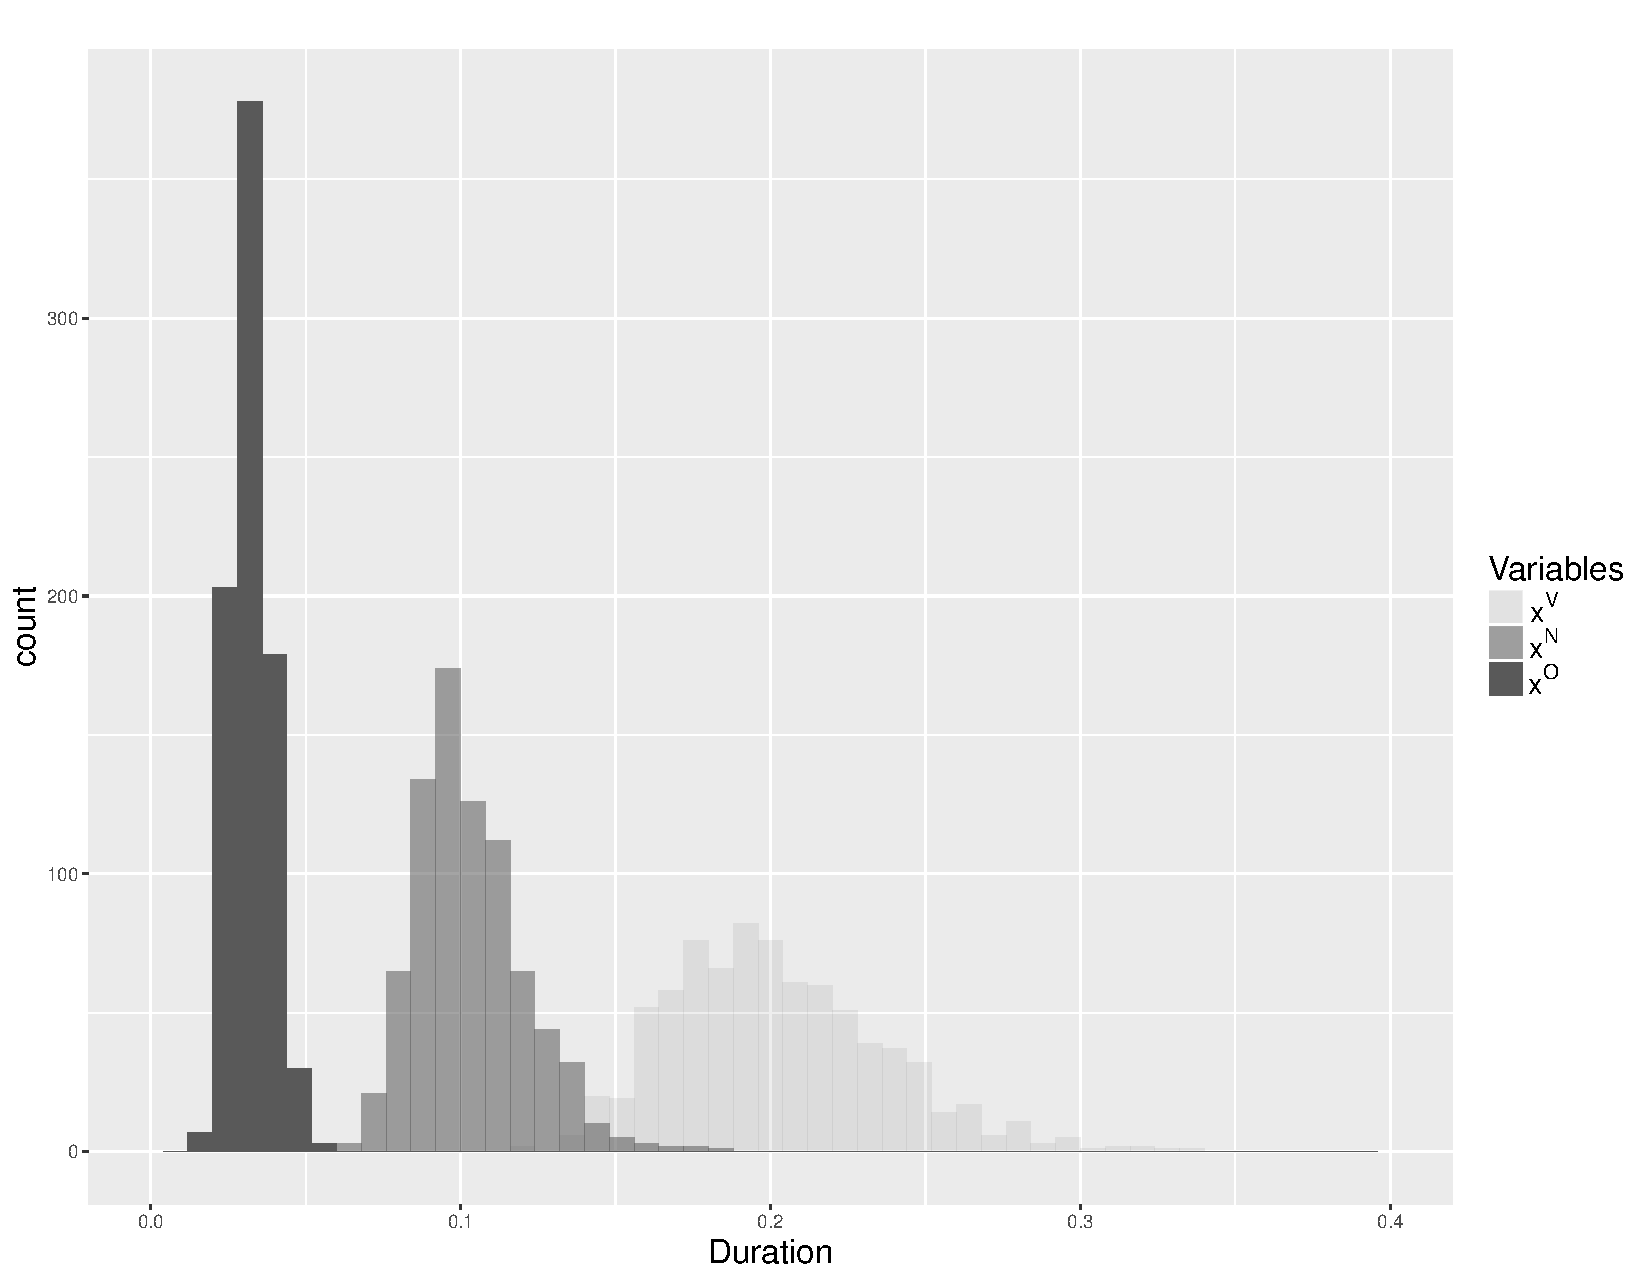
\includegraphics[width=0.3\paperwidth,bb = 0 0 200 100, draft, type=eps]{/Users/becca/Dropbox/CurrentWork/PerceptionProduction/VowelNasalization/SpeakingRateI10000.pdf}\caption{\label{fig:SpeakingRateOnly}Phoneme-Split Model: Speaking rate only}
\par\end{centering}
\end{figure}

With appropriately chosen constants, the speaking rate force is capable
of disrupting the influence of the frequency-based attractor. This
allows the equilibrium state of the model to vary as a function of
word frequency ($\beta$). For $T=x_{i}^{N}$, the fluency effect
acts consistently to shift the overlap longer ($T=x_{i}^{N}$). If
it is too weak ($\beta$ too small), then the speaking rate equilibrium
shown in Figure \ref{fig:SpeakingRateOnly} prevails. If it is strong
enough, then it is able to shift the overlap distribution to larger
values (rightward). This is possible because the speaking rate transform
depends on the current value of the overlap parameter for any given
token (expressed in the variable \emph{A} of Eq. (\ref{eq:Speaking rate transform})).
Figure \ref{fig:NasalizationModel1} shows the output of the model
with both speaking rate and frequency bias, run for three different
values of $\beta$. Note that the number of model iterations is essentially
arbitrary. Because the number is large (10,000), there is a reasonable
expectation that a stable state has been reached, but no tests of
convergence were performed. In this section we are more concerned
with the qualitative behavior of the model, and comparisons in which
all but one aspect of the simulations are kept constant.

\begin{figure}[H]

\subfloat[Low-frequency word ($\beta=.05$)]{

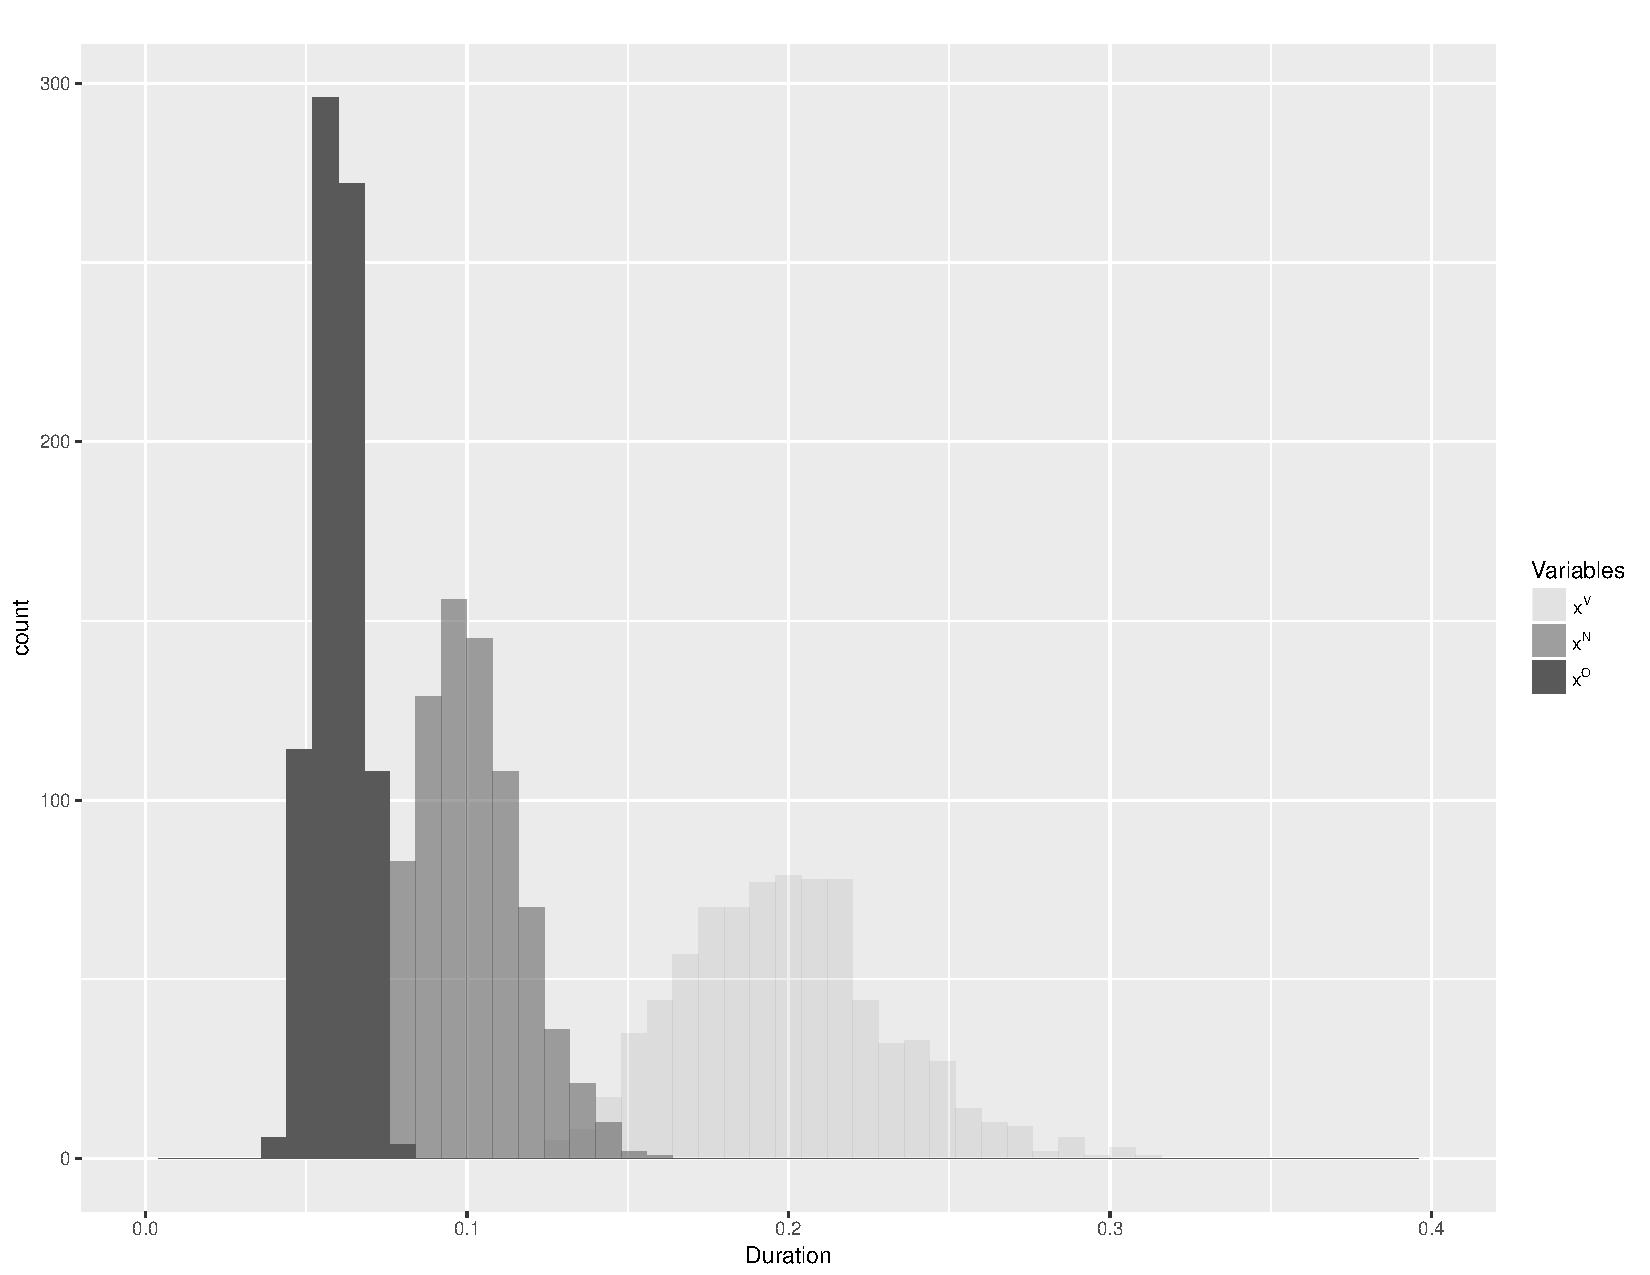
\includegraphics[width=0.25\paperwidth,bb = 0 0 200 100, draft, type=eps]{/Users/becca/Dropbox/CurrentWork/PerceptionProduction/VowelNasalization/SpeakingRateFrequencybeta=.05.pdf}

}\subfloat[Mid-frequency word ($\beta=.2$)]{

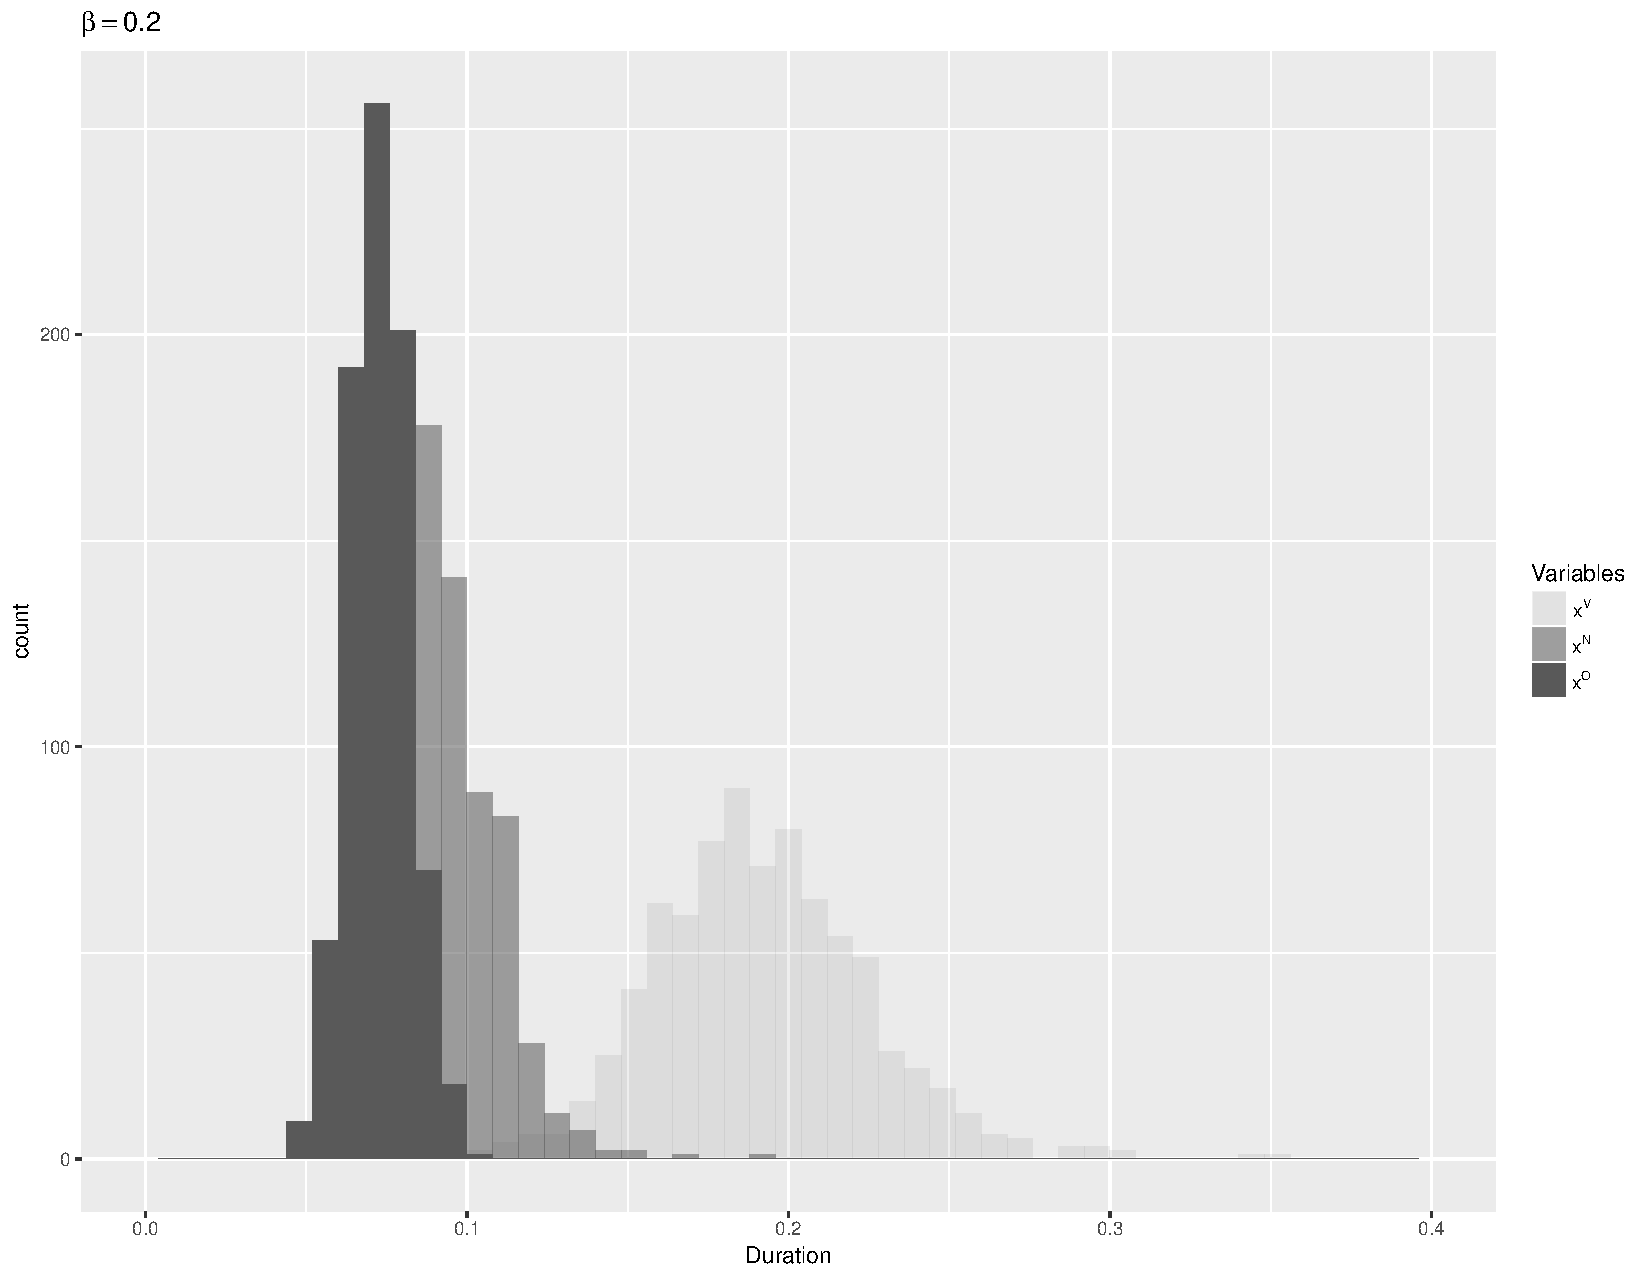
\includegraphics[width=0.25\paperwidth,bb = 0 0 200 100, draft, type=eps]{/Users/becca/Dropbox/CurrentWork/PerceptionProduction/VowelNasalization/SpeakingRateFrequencybeta=.2.pdf}

}\subfloat[High-frequency word ($\beta=.5$)]{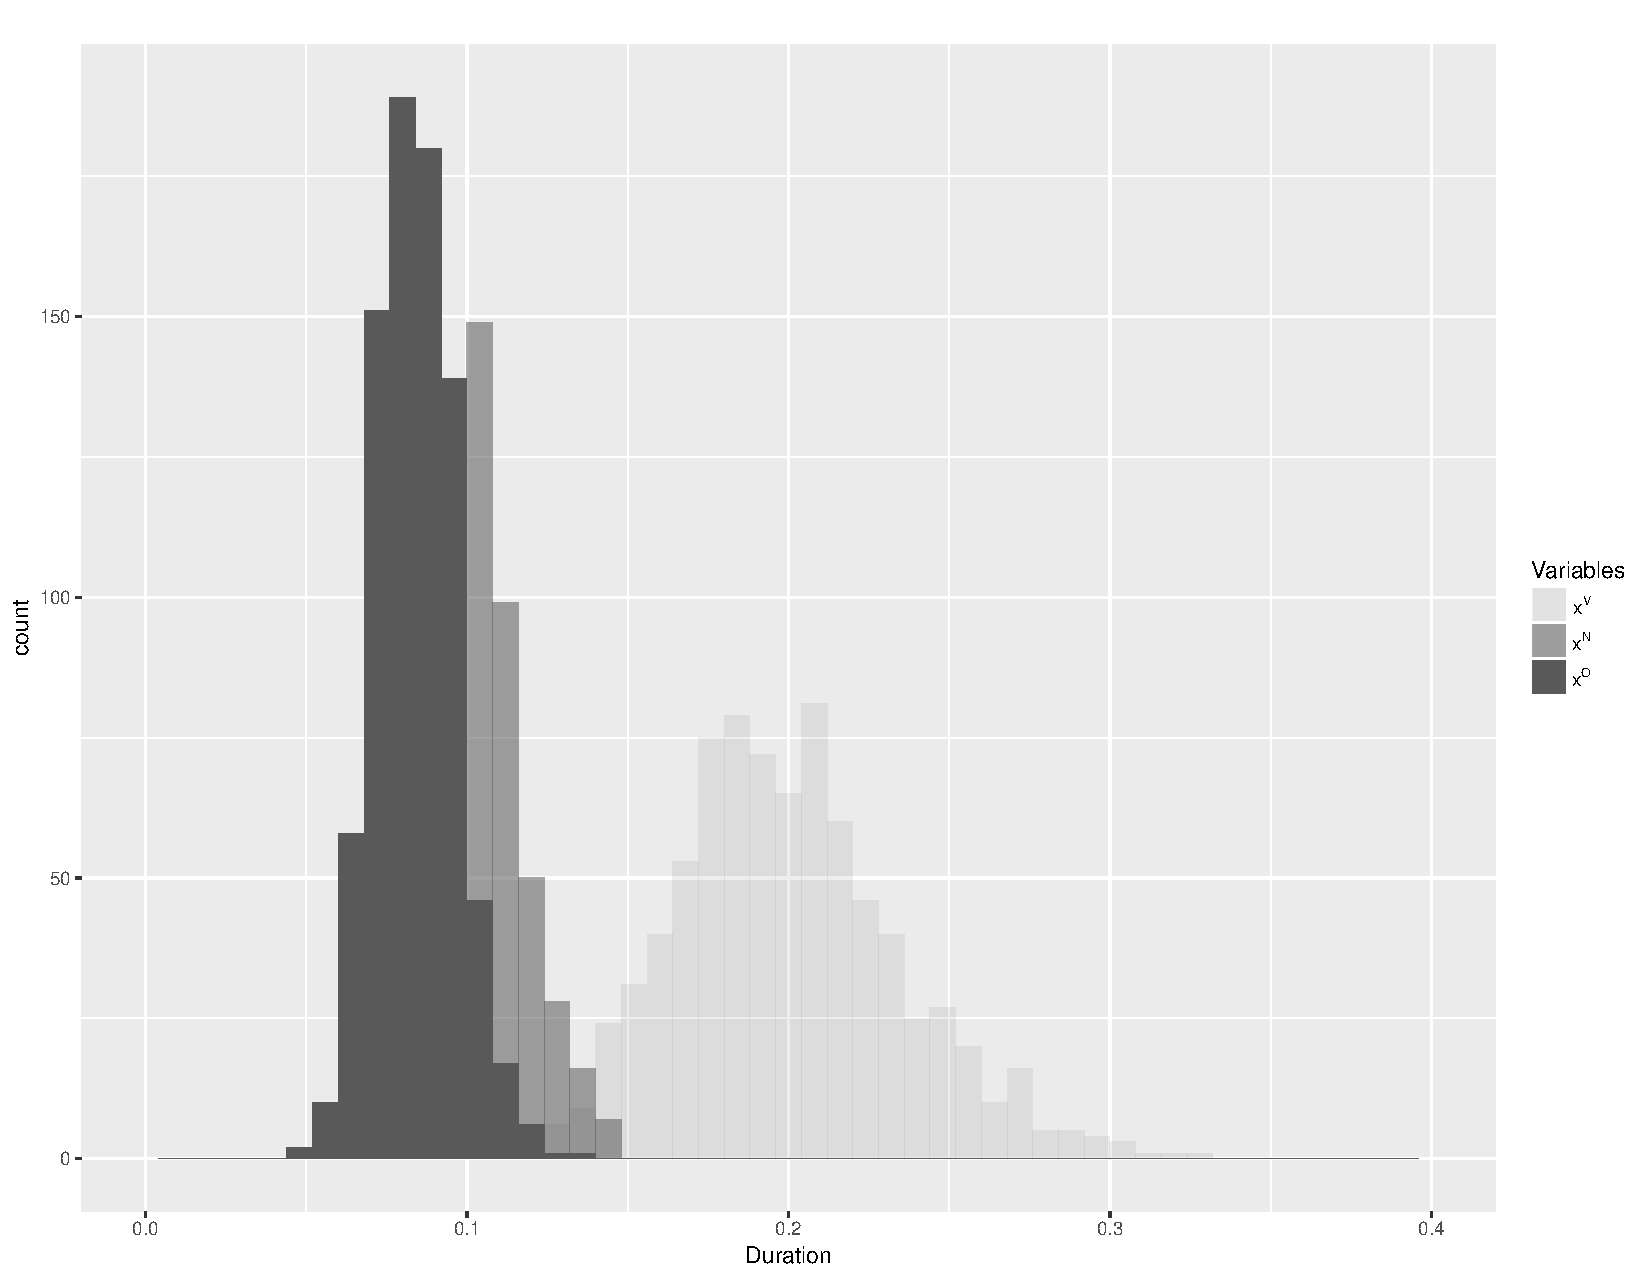
\includegraphics[width=0.25\paperwidth,bb = 0 0 200 100, draft, type=eps]{/Users/becca/Dropbox/CurrentWork/PerceptionProduction/VowelNasalization/SpeakingRateFrequencybeta=.5.pdf}

}\caption{\label{fig:NasalizationModel1}No-Phoneme Phoneme-Split Model (Frequency
Attractor). Each model run for 10,000 cycles from the same initial
distributions. }
\end{figure}

The No-Phoneme Phoneme-Split model predicts that words with higher
frequencies should be produced, on average, with vowels that are more
nasalized (larger degree of overlap between gestures), than lower
frequency words. It also shows that it is possible to achieve stable
phonetic change from a change in word frequency. The model implements
a theory of nasal vowel genesis as an emergent property of gradient
effects acting directly on articulatory parameters. Only in the special
case where overlap is roughly equivalent to nasal duration, would
the data likely be analyzed (by a linguist) as the result of phoneme
split. This state in the model, however, has no special status. And
distributions that appear intermediate with regard to the average
ratio of overlap duration to velum gesture duration can be stable.
Conceptualizing phoneme split in this way allows us to avoid the actuation
paradox that requires the loss of the conditioning environment, but
the retention of the conditioned allophone (see Chapter \ref{sec:Actuation-1}).
In fact, as there are no phoneme-level representations in this model,
there are no allophones, and no conditioning environments, in the
classical sense. Therefore, this model is also a demonstration that
phoneme-level representations are not necessary (nor is any misperception/misarticulation
pressure of the kind discussed in the previous Chapter), to achieve
a working model with the generally correct behavior. 

The source of the nasalization effect in this model is the coordination
between the tongue body and velum gestures. This parameter, however,
is part of the underlying specification of each word token. The No-Phoneme
model is thus a \noun{state} model. Arguably, a \noun{state} model
represents a change that has already taken place, in which a process
of nasalization has been reinterpreted as a static property of a unitary
representation. In the next sections we will turn to a \noun{process}
model of vowel nasalization, returning to the misperception/misarticulation
actuation mechanism. This will also involve introducing a sub-lexical
level of representation, and to revisiting the implementation of word
frequency.

\section{Parsing and Misparsing}

In order to recover the meaning of a given speech signal, it is necessary,
at minimum, to identify the individual lexical items present. This,
in turn, requires determining where one word ends and the next begins.
The highly context-sensitive nature of acoustic cues, as well as the
lack of consistent silence, or other markers, of the boundaries between
words or sounds, make this a computationally difficult task. And this
is not just an acquisition problem. Signal parsing, or segmentation,
is something that must be carried out every time speech is perceived. 

That segmentation of some kind must also take place at the sub-lexical
level is evidenced by a large literature on what are known as “trading
relations”, in which the value along a given phonetic dimension
that separates two members of a phonemic contrast is shown to vary
depending on the values of the other phonetic cues present. And those
other cues that influence the boundary location are not just those
that occur within the segment itself. For example, a given phone ({[t]})
may be ambiguous as to whether it belongs with a preceding or following
word (e.g., “great ship” {[}{ɡɹe͡ɪt}\#{ʃɪp}{]}
versus “gray chip” {[}{ɡɹe͡ɪ}\#{t͡ʃɪp}{]}),
and the actual word sequence that is heard will depend on the durations
of the surrounding segments; longer durations of {[e͡ɪ]}
increase the likelihood of “gray” over “great”, while
shorter durations of {[ʃ]} increase the likelihood of “chip”
over “ship”. An acoustic cue (such as silence itself) may also
be ambiguous as to whether it originates from a phoneme ({/t/})
or a break between words (“great ship” versus “gray ship”
{[}{ɡɹe͡ɪ}\#{ʃɪp}{]}; longer durations of silence
increase the likelihood of “great” over “gray” (\citealt{repp1978perceptual}).
An acoustic feature may also be ambiguous as to whether it belongs
to a preceding segment, a following segment, or both ({[}{ɹa͡ɪpbɛɹiz}{]}
as either “right berries” or “ripe berries”) (\citealt{Gow2003}). 

In all of the preceding examples the ambiguity exists because of the
existence of multiple real-word alternatives. Without those alternatives,
or competitors, phonetically ambiguous input quickly becomes perceptually
unambiguous (e.g., \citealp{warren1970perceptual,ganong1980phonetic}).
The strong susceptibility of low-level perception to high-level expectations
also speaks to the amount of noise, or essentially unpredictable variability,
in the acoustic realization of a given abstract category. Speech perception
involves the complex integration of multiple cues, each of which,
in isolation, may be relatively uninformative, in order to arrive
at a single parse, a single percept, of what is heard. This percept
is presumably the best alternative among those available to the listener
(see \citet{davis2007hearing} for a review of the literature). Although
speech perception appears extremely robust due to the fact that the
meaning intended by the speaker is usually recoverable by the listener,
that robustness is a property of the entire set of cues available,
not of acoustic features alone, and certainly not of individual acoustic
features. Rather than conceptualizing sound change as the relatively
rare event in which the listener mishears, or the speaker misspeaks,
it may be the case that what we typically think of as the “changed”
variants are already present within the distribution of stored tokens,
as one of multiple possible parses of each inherently ambiguous input
signal.

\section{Multiple Parses}

The classical way in which sound change is conceptualized is based
on the assumption that there exists a unique, correct, sub-lexical
representation for each word. It is meaningless to speak of phoneme-level
“errors” unless this is the case. Consider the following hypothetical
example (where \emph{$x>y$} indicates an historical change from \emph{x}
to \emph{y}):
\begin{covexamples}
\item \label{anpa>ampa}{anpa \textgreater{} ampa}
\end{covexamples}
(\ref{anpa>ampa}) is a common type of change known as nasal place
assimilation. In this example, the coronal feature of the nasal $/n/$
is assimilated to (or replaced by) the labial feature of the following
$/p/$. Speakers of a language that undergoes this change presumably
had an earlier allophonic rule specifying that $/n/$'s preceding
stops take on the place features of that stop. Therefore, the change
could only have occurred if they uncharacteristically failed to account
for this rule, or they made the “wrong” choice for a production
that was especially strongly assimilated. In either case, listeners
are assumed to parse their acoustic input into a sequence of discrete
phones, deciding for each segment whether to normalize or accept at
face value. Thus, for a change from {/anpa/} to {/ampa/}
to have actually occurred in the way it is denoted here, it must be
the case that listeners used to routinely segment continuous acoustic
tokens of this word into the sequence of units {/a/}, {/n/},
{/p/}, {/a/}, until they switched to segmenting
those tokens into the sequence {/a/}, {/m/}, {/p/},
{/a/}. 

Of course, we know that a discrete series of abstract symbols (either
{[anpa]} or {[ampa]} ) is not present in the acoustic
signal in any objective sense. The abstract notation also implies
that this change occurs once, simultaneously, for all words, and for
all word tokens. However, adopting the hypothesis that multiple experienced
instances of speech are stored implies that change would have to occur
over individual tokens. In fact, the multiple-parse hypothesis is
a logical consequence of the basic tenet of the exemplar framework.
The conflation of perception and production that we saw in in the
the exemplar models of Chapters \ref{fig:Feedback Loop} and \ref{sec:Models-of-Change}
is borrowed directly from the standard generative notation. Once a
transformation from perceptual tokens to production tokens is required,
it becomes clear 1) that parsing is necessary in the first place,
and 2) that it must occur for each experienced token. Recognizing
that acoustic tokens are inherently ambiguous with respect to their
decomposition into discrete units suggests, in turn, that variable
parses might be the norm rather than the exception\footnote{This is closely related to the proposal that stored lexical items
can have more than one representation (see, e.g., \citealp{hooper1976word,Janda2008,Bybee2001}).
Split representations are also assumed to be the outcome of discontinuous
articulatory change in the model of \citet{Garrett2013}.}. 

In the nasal assimilation example, there are two obvious alternative
parses, differing in whether they contain the phoneme $/n/$ or $/m/$,
thus the word-level category “anpa” is hypothesized to be composed
of at least some tokens specified with production targets for $/n/$,
and some for $/m/$. However, additional possible parses exist if
we do not assume the available phoneme inventory \emph{a priori}.
In fact, if we allow all universally possible segments into the analysis
space, then we avoid the actuation paradox of the classical diachronic
approach. As the next section will show, this re-framing of the change
question allows synchronic variation to be linked to diachronic change
in a way that is not dependent on either stopping or starting the
model at a critical point in time. 

\section{Representations II}

The Multiple-Parse model adds a \noun{process} component to the No-Phoneme
model. The process is implemented at the level of the articulatory
gesture, but conceptually requires the existence of abstract categories
intermediate between the word and the gesture. As before, the change
occurs in the distribution of variants that already exist, rather
than in the genesis of entirely novel forms. This aspect bears some
similarity to the proposal in \citet{Baker2011}, based on misanalysis
of the signal, but the current model is not abrupt, nor does it require
“extreme” variants to be adopted.

The conversion from perception to production is the locus of sub-lexical
parsing, mapping every continuous acoustic token into a series of
categorical units. In principle, these units can consist of any contiguous
set as long as it is phonetically plausible, and exhaustively parses
the input signal. However, in the case of vowel nasalization, we will
be concerned with two particular possibilities: the one-sublexical-unit
analysis, and the two-sublexical-unit analysis. These are of special
interest, of course, because they bear considerable similarity to
the classical analyses of the phenomenon before change (two units),
and after change (one unit). However, it is important to be very careful
in how these units are described, because the traditional notational
system essentially forces enforces an analysis more general than the
word level. In order not to assume generalization, and remain representationally
consistent, the following notation will be adopted for the two sub-lexical
parses of the word in question (“am”): $/\tilde{V}_{am}/$ (Analysis
1), and $/V_{am}/+/N_{am}/$ (Analysis 2). The desired implication
is that only after generalization across multiple words could something
similar to the abstract categories $/\widetilde{V}/$ and $/V/+/N/$
arise.

For the articulatory parameters already defined, a single-unit parse
means that all three values will be stored on the production side.
$/\tilde{V}_{am}/$ is a 3-dimensional cloud, and entrenchment applies
over each dimension (note that this is what was assumed for all tokens
in the No-Phoneme Model. Which, therefore, implicitly assumed a single-unit
analysis). The two-unit parse, however, is explicitly a \noun{process}
analysis, entailing that one token is drawn from a one-dimensional
\emph{$/V_{am}/$} cloud, one from a one-dimensional \emph{$/N_{am}/$}
cloud, with concatenation occurring at the time of production. In
other words, the overlap between the two gestures is not stored, but
determined online. 

\section{Multiple-Parse Phoneme-Split Model}

Either analysis is possible for any given token, but, critically,
depends on the acoustic properties of that token. In this set of simulations
it will be assumed that word-level categorization is correct, and
that the three duration quantities ($x_{i}^{V},x_{i}^{N},x_{i}^{O}$),
are accurately recovered in perception, although this is not critical\footnote{If the error term is symmetrical, then it will have no qualitative
effect on the model dynamics.}. Analysis 1, the single-segment analysis, is more likely to be selected,
the more highly overlapped the gestures that produced that token,
while Analysis 2, the 2-segments-in-sequence analysis, is more likely
for less overlapped gestures. The specific dependence is on the quantity
$Q_{i}=\frac{x_{i}^{O}}{x_{i}^{N}}$\emph{ }. Larger values of $x_{i}^{O}$
lead to larger values of $Q_{i}$, as do smaller values of $x_{i}^{N}$.
Selecting for large \emph{Q} thus selects both for larger overlap
and shorter word durations. That duration should correlate with number
of constituents is a reasonable hypothesis. It can also be hypothesized
that articulatory gestures will tend to be more tightly coordinated
within, than across, segments, if shared constituency promotes greater
merger\footnote{I am not aware of evidence for this specific relationship, but there
is evidence for different types of gestural coordination across different
domains: between the onset and nucleus of a syllable, versus the nucleus
and coda (\citealt{Browman1988,byrd1996influences}); and within,
versus across, morpheme boundaries (\citealt{Cho2001}).}. The probability of Analysis 1, $P(a=1)$, depends on \emph{Q} in
the following way (\ref{eq:segmentation-1}).

\begin{equation}
P(a=1)=Ae^{-b(1-Q)}-C\label{eq:segmentation-1}
\end{equation}
Probability increases with increasing \emph{Q} because of the negative
exponential in (\ref{eq:segmentation-1}). The largest possible value
for \emph{Q} is 1, therefore $1-Q$ is always positive. When $Q=1$
, $P(a=1)$ reaches its maximum at $A-C$. How quickly the probability
decreases as a function of decreasing \emph{Q} is controlled by the
variable \emph{b. }The larger \emph{b}, the larger the negative exponential,
and the more quickly $P(a=1)$ decreases, selecting for larger mean
\emph{Q} values (and fewer tokens). See Appendix \ref{chap:Appendix E}
for additional details.

If Analysis 1 is chosen in perception, based on the value of $P(a=1)$,
then all three values of the token are stored. If Analysis 2 is chosen,
then the duration of the tongue body gesture ($x_{i}^{V}$), and the
duration of the velum gesture ($x_{i}^{N}$), are each stored in separate
categories, and the overlap value is discarded. Figure \ref{fig:MultiParse-Reps}
provides a schematic depiction of these relationships. Note that the
dimensions are not accurately represented here; two dimensions are
used for all categories to make the membership relationships easier
to see. Individual tokens are drawn as schematic gestural scores:
extent represents time, and fill type represents active articulator.
The horizontal alignment of the two bars in the tokens of the category
are meant to indicate the stored gestural overlap parameter. The thin
lines drawn between tokens of the and sub-categories indicate that
they are stored together, and will be produced together. Overlap must
be determined via a separate distribution. Entrenchment happens only
within individual sub-lexical categories\footnote{If entrenchment at the word-level is added it will have the effect
of pushing values back towards the means of the Analysis 2 categories,
since the model is initiated with those values, and the Analysis 2
parse is always more likely. }.

\begin{figure}[H]

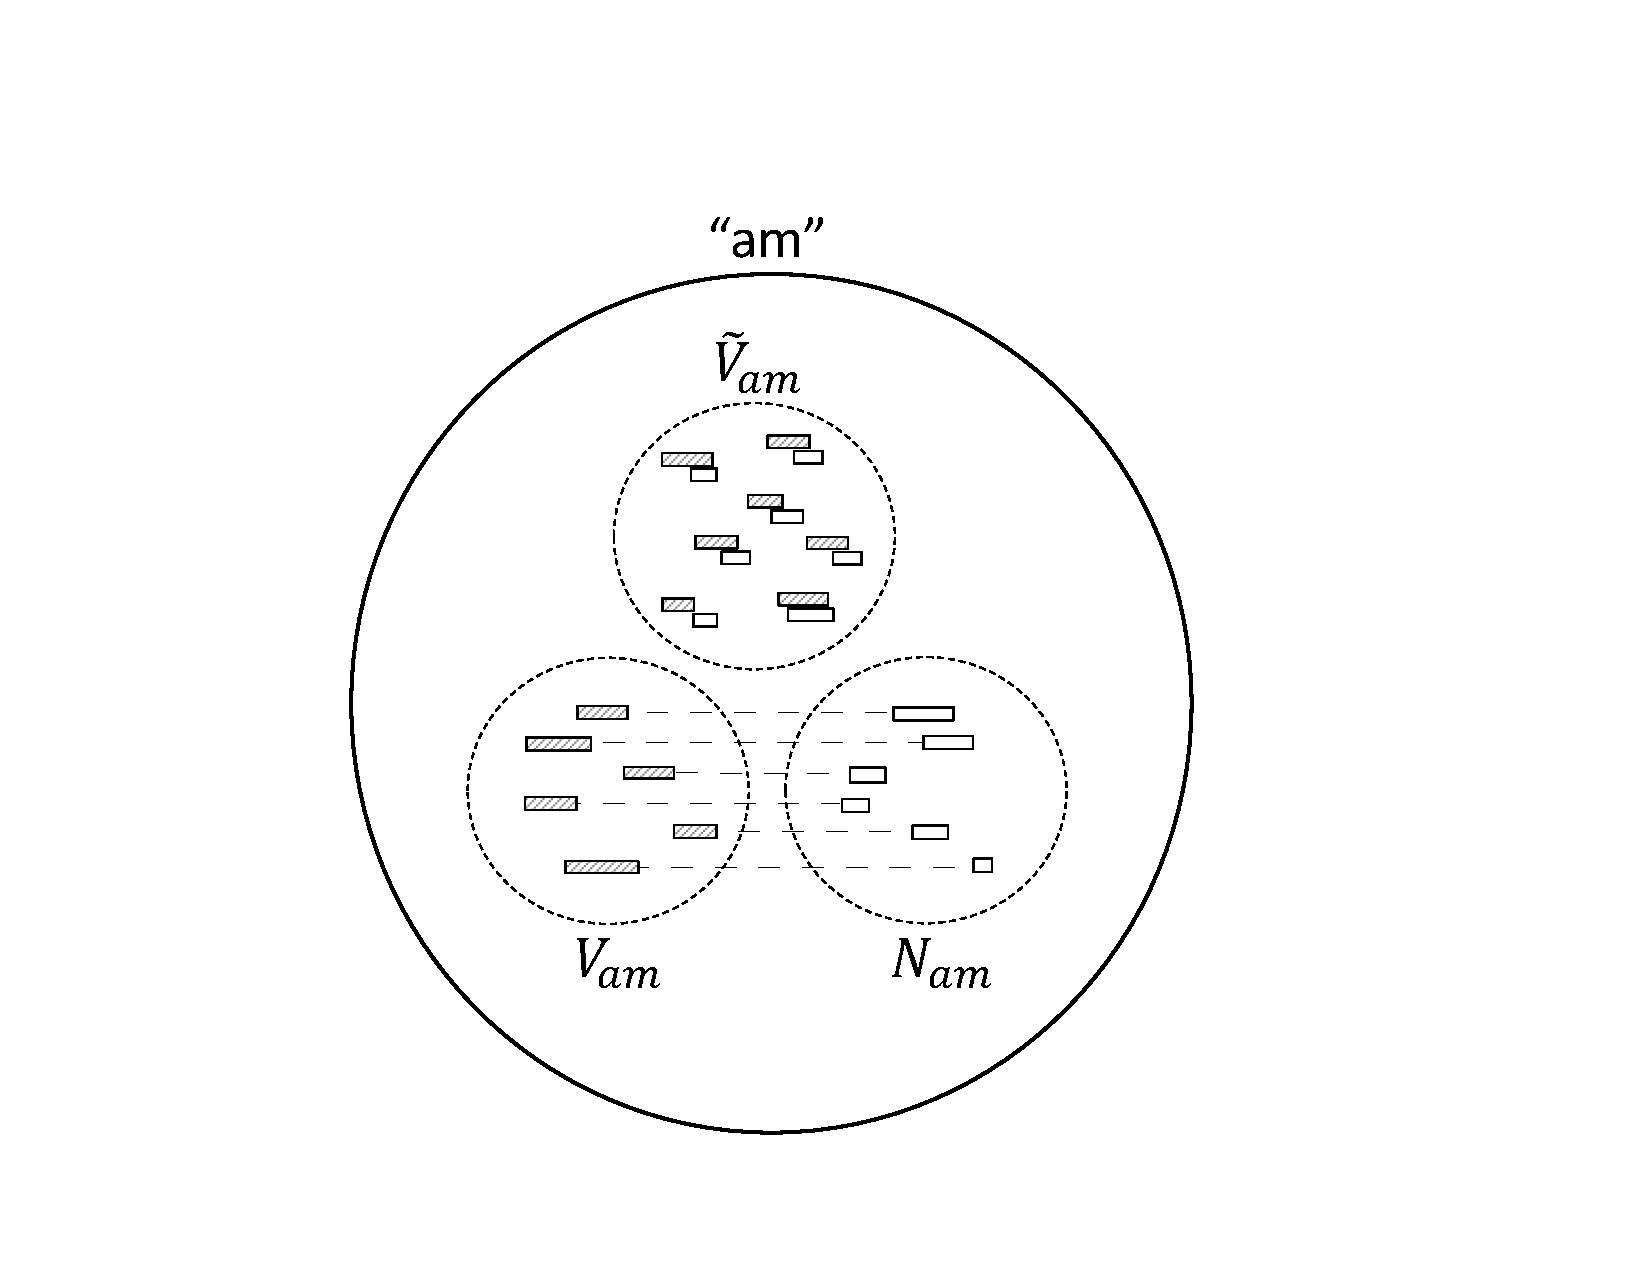
\includegraphics[width=0.75\textwidth,bb = 0 0 200 100, draft, type=eps]{MultiParseModel.pdf}\caption{\label{fig:MultiParse-Reps}Schematic depiction of the relationships
between the word-level category (“am”) and the sub-lexical level
categories of its constituents. Production-side representations.}

\end{figure}

Tokens are chosen randomly for production from among all stored values.
Once selected, the token is subject to the same speaking rate transformation
used in the No-Phoneme model. The overlap degree for an Analysis-2
token defaults to a fixed percentage of the current average value
of $x^{N}$ (with some variance). There is no phonetic bias in this
model. The selection bias that drives the feedback loop resides in
the choice of underlying analysis – the parsing of the input signal.
Eq. \ref{eq:segmentation-1} selects for large values of $x^{O}$,
and for small values of $x^{N}$, both of which will increase the
size of \emph{Q}, and thus increase the probability of Analysis 1.
There is no cumulativity such that these values grow more extreme,
but there is a constant pressure to sort tokens with the largest overlap
proportion into this sub-lexical category. Thus, if an independent
mechanism resulted in an increase in \emph{Q} for some tokens, those
tokens would raise the average \emph{Q} value of the $/\tilde{V}_{am}/$
sub-category.

A mechanism that shortens word duration will have this effect: shortening
$x^{N}$ (and $x^{V}$), and lengthening $x^{O}$. If higher frequency
is taken to result in faster productions, then an increase in frequency
would lead to more, and higher-valued \emph{Q}, tokens. For the simulations
reported below, frequency was implemented as a negative perturbation
to the mean value of the expansion force distribution. As a result,
higher frequency (higher resting activation) results in shorter words,
and thus shorter tongue body and velum gestures (and longer overlap)
under all speaking rates. This implementation will be discussed in
more detail in the following section. 

Figure \ref{fig:Multiple-Parse-Results} shows the model results as
a function of frequency. Each point is the result of running the model
for 10,000 iterations. Mean values for the three duration parameters,
as well as the proportion overlap (\emph{Q}) are given for each of
the categories: Panel 1: word-level; Panel 2: Analysis 1 tokens; Panel
3: Analysis 2 tokens. Note that the overlap proportion in Panel 3
shows the constraint that overlap proportion stay fixed with respect
to $\overline{x^{N}}$. Whereas, in Panel 2, as resting activation
(frequency) increases, the proportion overlap increases. Because the
number of tokens parsed into the $/\tilde{V}_{am}/$ category also
increases with increasing resting activation (from approximately 31\%
to 50\%), the overlap proportion increases for the word-level category
as a whole (Panel 1). 

\begin{figure}[H]
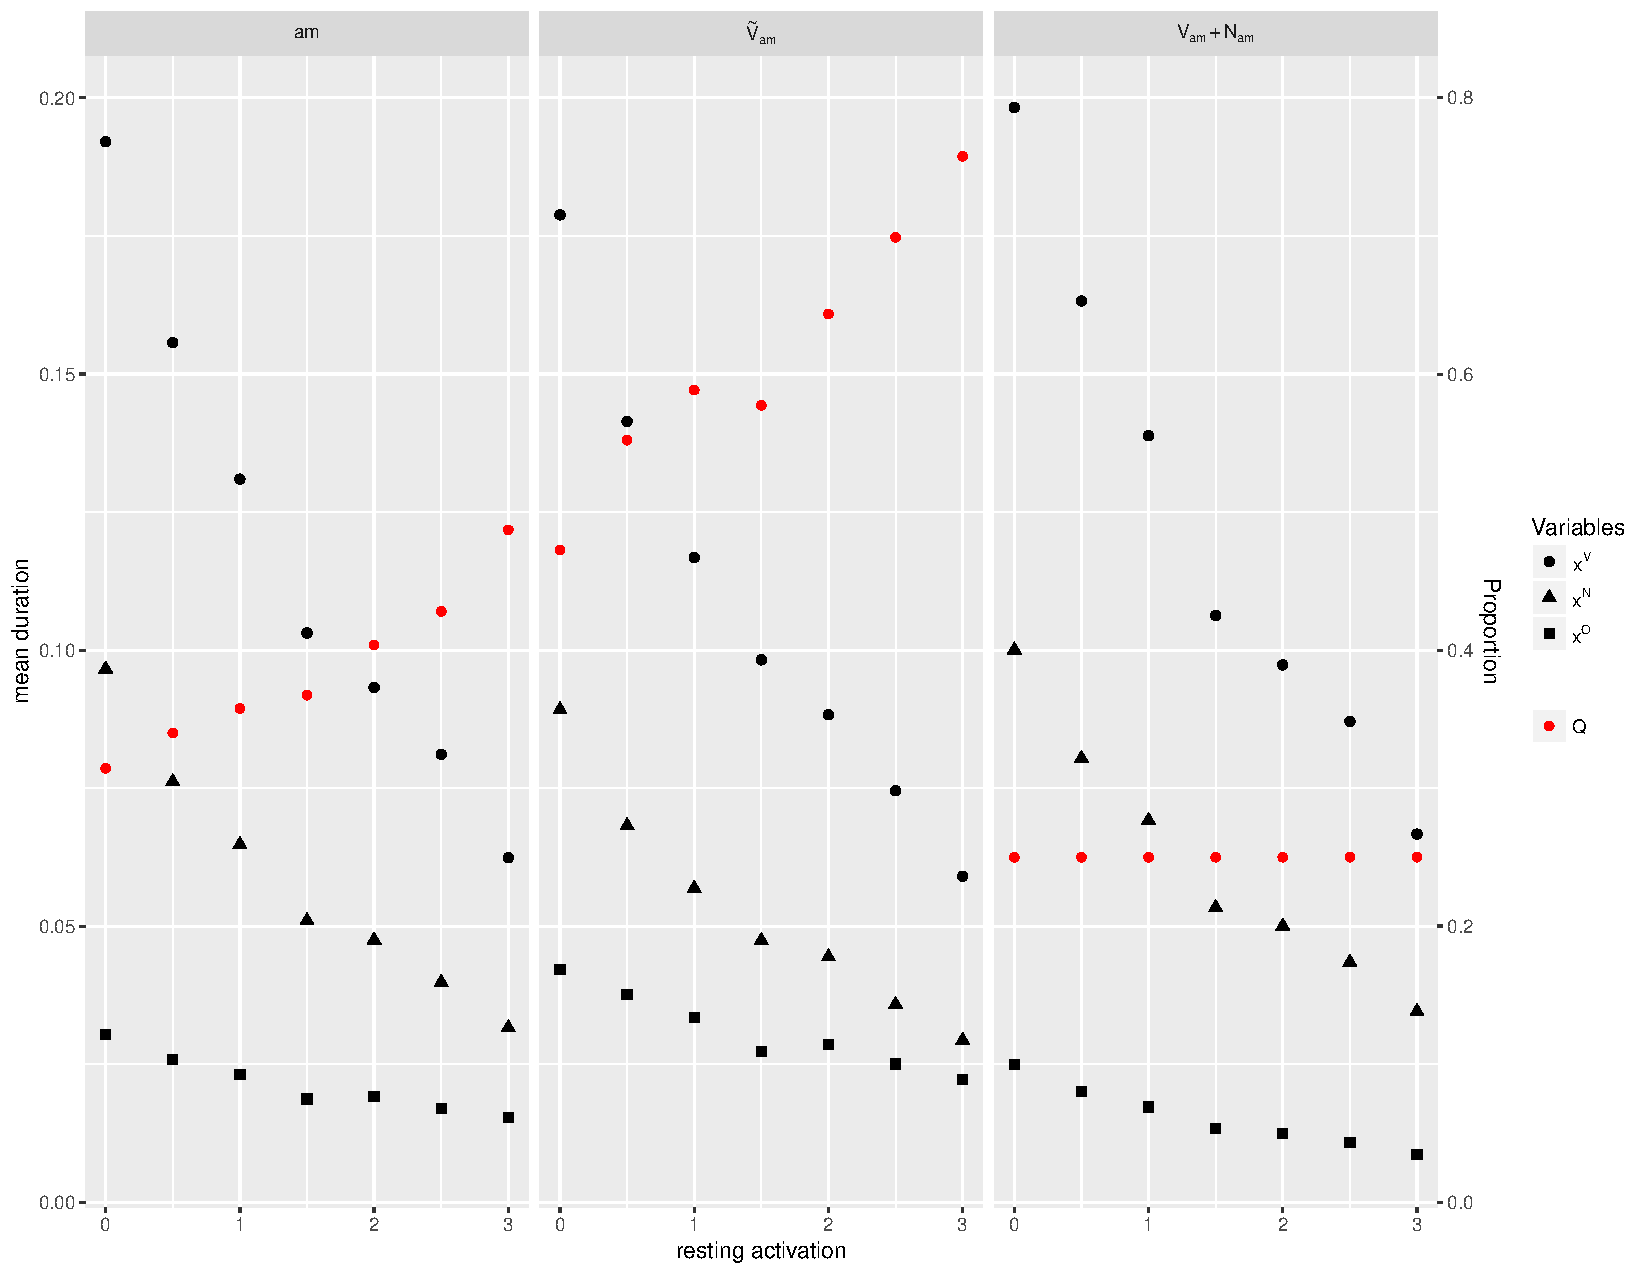
\includegraphics[width=0.75\textwidth,bb = 0 0 200 100, draft, type=eps]{/Users/becca/Dropbox/CurrentWork/PerceptionProduction/VowelNasalization/MultipleParseResults.pdf}\caption{\label{fig:Multiple-Parse-Results}Multiple-Parse Model: Results as
a function of resting activation (word frequency). Each point corresponds
to the mean after 10,000 model iterations. Mean articulatory durations
are plotted in black. Proportion overlap ($Q=\frac{\bar{x}^{O}}{\bar{x}^{N}}$)
is plotted in red. Panel 1: all word tokens; Panel 2: Analysis 1 tokens
only; Panel 3: Analysis 2 tokens only.}
\end{figure}


\section{\label{sec:Frequency-II}Frequency II}

In the No-Phoneme Phoneme-Split model frequency was implemented as
a fixed attractor on overlap duration (Section \ref{sec:Frequency-I}).
The assumption was that there existed an optimal (most fluent) production
of a given word with precisely the degree of gestural overlap given
by the attractor target. At the same time, in order to generate productions
that more closely resembled nasal vowels, it was necessary to set
the target quite high – in the reported simulations it was set to
the entire duration of the accompanying velum gesture. However, it
is not clear why the optimal production of the 2-gesture word should
exhibit such a large degree of overlap. And, in general, there is
no clear reason for greater practice, or increased fluency, to always
result in shortened, or reduced, articulations, especially to the
point where distinctiveness may be lost at the word and/or phoneme
level. Yet this seems to be the case with frequency effects. It has
been shown, for example, that individual segments within high-frequency
words are shorter, and that there are more likely to exhibit “deletions”
(dropping, or masking of a consonant, or unstressed vowel) (e.g.,
\citealt{Bell2003,Raymond2006,Bybee2008}). The realizations of segments
in higher-frequency words tend also to be less extreme, or more “centralized”,
perhaps failing to reach the usual articulatory target (e.g., \citealt{munson2004effect,Scarborough2004,gahl2008time}).

The listener-based account of frequency effects explains these phenomena
as a consequences of contextual predictability. It is actually the
less predictable, less easy to access, more confusable, forms that
are produced with particular care (hyper-articulated) by the speaker
in order to aid intelligibility (e.g. \citeauthor{Aylett2004}). In
the absence of that pressure, articulations are reduced to the degree
possible, facilitating the task of the speaker. Factors that have
been shown to affect predictability, as well as word form, include
sentence, or discourse, context, bigram frequency, and unigram frequency,
among others. Nevertheless, there are a number of results that are
not compatible with a strictly listener-based theory, studies that
have shown that speakers do not always alter their productions in
such a way as to facilitate listener comprehension (see \citet{turnbull2015assessing}
for a review of the literature).

As mentioned briefly in Chapter \ref{subsec:Word-Frequency}, the
speaker-based approach attributes frequency effects to automatic production-side
mechanisms. This is usually couched in terms of activation levels,
within some kind of lexical network model where different representations
“compete” in both perception and production (e.g., \citealp{mcclelland1981interactive,Dell1986}).
In terms of word retrieval, the successful candidate is the one that
achieves a given threshold of activation first. Every time a word
is accessed, or produced, it is activated to this level. Repeated
activations, within some time period, are taken to result in some
level of residual activation that persists even when the word is not
selected. This “resting” activation level is naturally higher
in higher frequency words, giving them a head start against lower-frequency
competitors. 

The resting-activation account is in line with results establishing
that higher-frequency words are produced earlier than lower-frequency
ones in a variety of tasks, such as picture naming, and word or sentence
reading – even with delays. Higher-frequency words also lead to faster
response times in lexical decision and other speeded response tasks,
as well as to greater accuracy in word recognition (e.g., \citealt{howes1951visual,balota1985locus,Luce1986,Marslen-Wilson1990}).
However, it is not at all obvious that higher resting activation alone
can account for articulatory or temporal reduction (hypo-articulation).

In fact, it has been argued \emph{both} that a higher activation level
should lead to hyper-articulation (e.g., \citealt{Baese-Berk2009}),
and that it should lead to hypo-articulation (e.g., \citealt{gahl2012reduce})\footnote{Note that different results were obtained in these studies, one based
on laboratory data, and one on conversational corpus data.}. In works that adopt the latter position the connection seems to
be assumed. For example, \citeauthor{gahl2012reduce}(2012: p.79)
write that “Production-based accounts...would lead one to expect
that words that are retrieved quickly tend to be phonetically reduced
– \emph{provided that fast retrieval speed translates into fast production
speed”} (emphasis mine).

The fact that there does not appear to be a well-worked out mechanism
for this result raises the possibility that we have yet to find the
right model for frequency. Empirically, however, the correlation between
shorter/faster productions and higher word frequency seems quite robust.
In the Multiple-Parse Model, a frequency-based increase in production
speed is taken to be an additive effect, acting to effectively shift
the speaking rate distribution. If we continue to assume that speaking
rate acts independently of other model forces, then words will continue
to be pulled in both directions, expanding or compressing in turn.
Subject to the same large positive force, both low and high frequency
words will be produced more slowly, and will thus be longer than if
no force had applied. However, the high-frequency word will be somewhat
shorter than its low frequency counterpart, due to the difference
in its resting state. The same will be found under compression (unless
floor is reached).

The dependence on frequency (resting activation) in Figure \ref{fig:Multiple-Parse-Results}
shows the effect of progressively shifting the speaking rate distribution;
shorter average word durations result in shorter $x^{N}$, and longer
$x^{O}$, and thus lead to a greater proportion of Analysis 1 tokens\footnote{Because the duration of overlap cannot exceed the length of the shortest
gesture, the longest \emph{absolute} overlap durations can only occur
with the longest word tokens, thus there is also some selection pressure
towards longer $x^{N}$ inherent in the $x^{O}$ measure. Reducing
the length of $x^{N}$ will therefore eliminate some of the largest
$x^{O}$ tokens.}. This shift is not unbounded, because speaking rate is a bi-directional
force; high-frequency words can also be lengthened, just not lengthened
quite as much as their lower-frequency counterparts. Note that the
frequency effect in this model acts on all tokens, both stored and
generated. In the latter case, we must assume that some type of motor
plan involving the concatenation of $/V_{am}/$ and $/N_{am}/$ is
associated with a resting activation value that affects the duration
of the resulting word. 

\section{Actuation }

As in the No-Phoneme Phoneme Split model, there is no single moment
at which a sound change occurs in the Multiple-Parse Phoneme-Split
Model. Every instance of perception involves a decision about parsing
which is based on existing synchronic variation. And every available
parse is a possibility at any time, for any token; it is the probabilities
of those parses which change over time. Although the nasal vowel parse
is assumed in the sense that it is one possible analysis for a given
token, this model, in fact, avoids many limiting assumptions about
the nature of sound change inherent to the classical view. For example,
the \emph{/V+N/} analysis is not privileged, beyond having a higher
probability of selection, given the starting distribution. Additional
analyses can be added to the set of parsing hypotheses, if motivated
by general-purpose properties of speech perception. It is consistently
the word level at which all forces act in this model, and at the level
of articulatory gesture that changes are realized. In particular,
this model does not rely on the allophonic level at which the synchronic
rule, and the diachronic change, are assumed to occur. As a result,
the normalization/lack of normalization question becomes a basic element
of speech processing: the analysis that must occur when perceptual
values are transformed into production values. 

If classification occurs at the word level, and words have articulatory
representations something like gestural scores, then it is not necessary
to first identify a series of abstract phonemes in order to identify
individual words. Thus, the problem of “compensating” for (the
feature of) nasalization at the level of the phoneme disappears. The
ambiguity remains regarding the proper articulatory realization of
a given acoustic input, but there is no longer a unique, correct sub-lexical
analysis. The possible analyses available to the listener, based on
their phonetic experience, should always include, at minimum, both
the “normalized” option, as well as the “unnormalized”
one.

In the specific simulations reported in the previous section, the
average percentage of the velum lowering gesture that occurred simultaneously
with the tongue body gesture varied from 30\%, for the lowest frequency
word, to about 50\% for the highest-frequency word. It was also the
case that the absolute gesture durations were considerably shorter
at the higher frequencies. These results describe a diachronic change
under the scenario in which a single word comes to be used more, or
less, frequently over time. Under the scenario in which frequencies
are fixed, but there exists a set of words with a range of different
frequencies, these results describe a synchronic distribution. The
model thus generates at least two testable predictions: 1) that a
difference in the degree of vowel nasalization should be observed
across words of different frequencies (provided the relevant phonological
context is sufficiently similar among those words), and 2) that the
highest-frequency words should approximate the degree of vowel nasalization
observed in languages that are described as having phonemically nasal
vowels. In other words, no exaggeration, or enhancement, of the effect
is required in this model. Lexicon-wide change is assumed to start
with change at the individual word level.

It is widely acknowledged that change (of certain kinds, at least)
happens on a word by word basis (e.g., \citealt{Phillips1984,Bybee2002,Pierrehumbert2002}),
and that some words can be `further along' in the change than others.
With regards to nasalized vowels in particular, \citet{malecot1960vowel}
offers evidence that the distinction between English words like “cap”
and “camp” is primarily that between a nasal and oral vowel
({[kæp]} vs. {[kæ̃p]}), rather than the presence
versus absence of a nasal consonant ({[kæp]} vs. {[kæ̃mp]}).
The English segmental inventory is not usually analyzed as containing
an abstract nasal vowel (although see \citet{Sole1992} for an argument
that nasal vowels are phonologically specified). Nevertheless, individual
tokens, or individual words, or even classes of words, may have phonetic
realizations that are indistinguishable from those generated from
an underlying nasal vowel. 
